\documentclass[12pt,journal,compsoc]{D:/Магистратура/English/bare_conf/IEEEtran}
\newcommand\MYhyperrefoptions{
pdfpagemode={UseOutlines},plainpages=false,pdfpagelabels=true,
colorlinks=true,linkcolor={black},citecolor={black},urlcolor={black},
pdftitle={Working with attached to repair documents in the system of automatic registration of repairs},
pdfsubject={Typesetting},
pdfauthor={Arseny Zorin}}
\usepackage{graphicx}
\graphicspath{{D:/Магистратура/English/bare_conf/}}

\begin{document}
\title{Working with attached to repair documents in the system of automatic registration of repairs}

\author{Arseny~Zorin}
\maketitle

\IEEEpeerreviewmaketitle



\section{Introduction}
\IEEEPARstart{S}ince the appearance of computers, progress isn't standing still. Technology has enormously improved in last decade. Among trends that appear one can find an ambient wireless Internet access to printing prosthesis on 3D printers or cloud storages. The latter became storage de-facto standard for past few years. It is used not only for private, but also for corporates document storing and data archiving.

The object of research is the authorized service center (ASC) that provides warranty and paid repair of household appliances. There are four branches situated in different parts of the city that take equipment for repair. Each repair operation performed by ASC produces an number of attached documents, their names equal to the ticket number:
\begin{itemize}
\item A photo of schild from back of equipment. This file is stored in a common folder for schilds' photos of this manufacturer.
\item A scanned warranty ticket. This file is stored in a common folder for scanned documents of this manufacturer.
\item An outbound repair receipt. Produced in case the repair was carried out at the client's residence. This file is stored in a common folder of outbound repairs for this manufacturer.
\item Various acts provided to a client including a technical condition act, a non-repairable act, a replacing device act.
\end{itemize}

All document folders are stored at branches offices and at the head office server. Data is transmitted between branches and the head office through FTP protocol.

This work was motivated by a need for modernization of tools for documents storage and transmition. The software programming language was C\# instead of VBA. For scanning documents and making photo of them new libraries will be used. All documents storage were moved to the cloud. Data will be stored and treated at the distributed servers in network. While using cloud storages, users have a possibility to access the data from different places and from different devices which have an Internet access. Also cloud storage can prevent losing information in case of failure of a local storage.

\section{Practical implementation}
\subsection{Working with AForge.NET}
\IEEEPARstart{T}aking photo of a schild: after the button pressed, a new window with video player element will open. Stream video from selected web-camera will be played on this element. After the button "Take a snapshot" pressed, there will be capture of the picture from video player element and an obtained picture will be stored in the specified directory in .jpg format. 

The .NET Framework does not support working with web-cameras it means that there is no video playback element. However, there is namespace AForge.Controls with VideoSourcePlayer element in AForge.NET. This element was created only for using in Windows Forms software. The decision of developing software with using WPF was taken and there are few methods of solution:
\begin{itemize}
\item The creation of a hybrid application. In addition to the WPF window, there will be one Windows Forms window.
\item Using a WindowsFormsHost element. This element allows to place Windows Forms element on WPF page.
\end{itemize}

The latter variant was selected. Forits realization we have to add: System.Windows.Forms.Integration and AForge.Controls namespaces, WindowsFormsHost element and VideoSourcePlayer inside it (Fig. 1).
\begin{figure}[h]
\centering
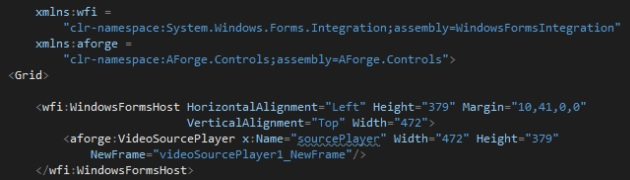
\includegraphics[width=0.5\textwidth]{1}
\centering
\caption{Adding namespces and elements}
\end{figure}

In addition to the playback element we have to add elements for interaction with VideoSourcePlayer element:
\begin{itemize}
\item "Take a snapshot" button
\item List of playback sources
\end{itemize}
After addition of all elements, the window in "Constructor" mode will looks like on fig. 2.
\begin{figure}[h]
\centering
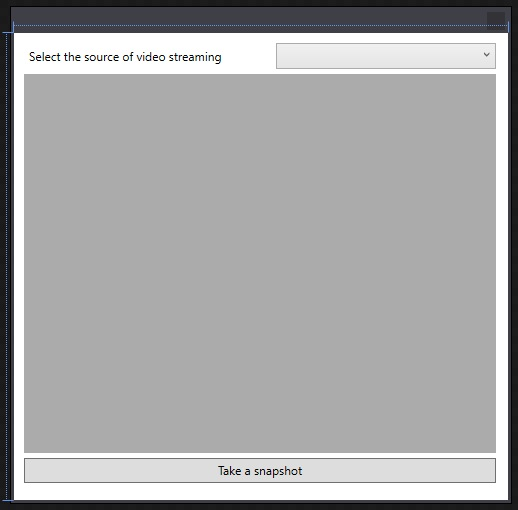
\includegraphics[width=0.4\textwidth]{2}
\centering
\caption{Window view in the constructor mode}
\end{figure}

There is the AForge.Video.DirectShow. VideoCaptureDevice class for capturing video from an input-output (I/O) device. It is necessary to set device's moniker (the name of a cpecific instance of an object. It is a COM-object that has its own way to create and maintain a special interface - IMoniker), which will capture the picture. In addition, we have to add event handler NewFrame. Every time new frame will be received, this event will raise. Received frame sends to the handler in the Bitmap format. It can be processed and stored in the specified format in the right place.

The list will be filled with names of all connected I/O devices and the default device will be the first in the list.

The event comboBoxSources\_SelectedIndexChanged rises after changing selection of source. It stops streaming from previous I/O device, set a moniker to the VideoCaptureDevice class of a new selected device and resumes streaming.

Pressing the button "Take a snapshot" changes the value of the take\_pict boolean variable on true. The value of this variable checks in the event raised after receiving of a new frame. If its value equals to true, then received image saves in .jpg format in specified place. In our case - Yandex.Disk.

The method EndOfWork, that stops streaming and frees used resources, is called after after closing the window.

\subsection{Working with TWAIN library}
We need to program a button for documents scanning. There will be selection of data sources after clicking on the button (if there are several connected scanners). After selecting of the source, scanning will start and received file will be stored at the specific folder in .jpeg format. We have to close data source after finishing the scanning.

There are a lot of different methods in the TWAIN library. However, only several of them will be used for completing the task:
\begin{itemize}
\item OpenDataSource() - Opens a data source. Type of return value - bool. Value true if operation is successful, else - false. 
\item SelectDataSource() - Shows dialog window for selecting a data source. Type of return value - bool. Value true if operation is successful, else - false.
\item Property ShowUI - Gets or sets a value indicating wether to show user interface (UI) of TWAIN-source (to speed up value sets as false)
\item Acquire() - Gets an image from a data source. Type of return value - void. 
\item GetImage(int index) - Returns a scanned image. The parameter index - index of return image. Type of return value - System.Drawing.Image. 
\item CloseDataSource() - Closes a data source. Type of return value - bool. Value true if operation is successful, else - false.
\end{itemize}

The platform of developed software was changed to 32-bit(x86). The reason is that 64-bit(x64) platform is not supported with all scanners.

\subsection{Working with Microsoft.Office.Interop}
For beginning the work with Word and Excel documents from Visual Studio, it is necessary to add references into the project: Microsoft.Office.Interop.Word and Microsoft.Office.Interop.Excel. 

\subsubsection{Working with Microsoft.Office.Interop.Word}
The words starting wigth \@ must be replaced with values of table cells during the creation of acts. Application object, which is the parent of all objects, used for working  in the .NET. The work with its methods and properties is available after the reference on this object was received. This object provides a big set of methods and properties that allows to manage the Microsoft Word. Particularly all Word functions require an object parameters.

There are two important moments about working with Word throug C\#:
\begin{itemize}
\item An unmanaged resource is created. It is a separate process in memory with Word application. This process will not be collected with garbage collector. If it will not be closed and showed on the screen it will be remained in the computer memory untill turning off. Such processes acumulate invisibly for the user. The programmer must to take care of closing the unmanaged resources.
\item Word runs invisible by default, we need to display it ourselves.
\end{itemize}

Despite the latter fact, in our case, Word document will be invisible for the user. However, EndOfWork method will close this process.

Object Range - the main object for working with Word. This object is the region in the document and can include a pair of characters, tables, bookmarks etc. There is Selection object - part of document selected with pointer, that can be converted into the Range. For task execution we have to get Range for the whole document, then to find necessary string in received Range, get Range for this string and inside the latter Range to change the text on required.

There is a rare error in the Microsoft.Office.Interop library that was accepted by Microsoft company. The error is exiting Execute method from Find interface with "Stub received bad data" error. The reason is using Globally Unique Identifiers (GUIDs) in Word that were used in Excel 95. These identifiers begin to specify on Excel library if Excel 95 library was registered later than Word library. It causes to incorrect construction of proxy v-table for out-of-process clients. As a result, queries to that table causes or an error a failure, because instead of sending to the Wrod they are sending to the Excel.

Standard search and replacing a string with Interop.Word.Find (Fig. 3) interface must be replaced with using library System.Reflection (Fig. 4).
\begin{figure}[h]
\centering
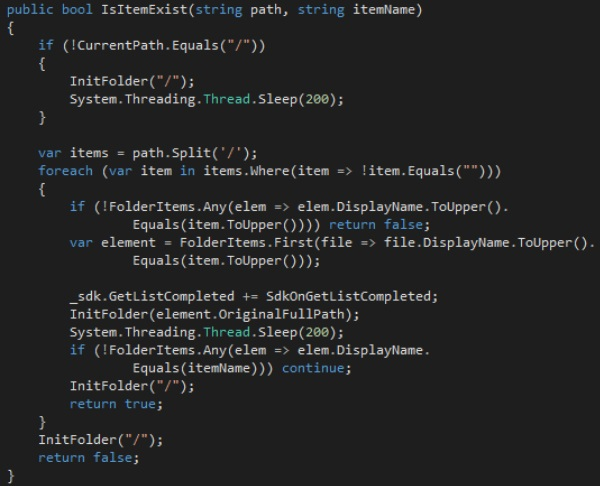
\includegraphics[width=0.5\textwidth]{3}
\centering
\caption{Searching and replacing a string}
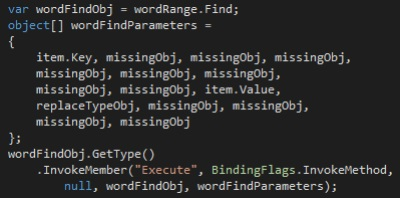
\includegraphics[width=0.5\textwidth]{4}
\centering
\caption{Replaced part of the code}
\end{figure}

When a work with template is over, it is printingwith standard method PrintOut. In some cases filled template must be saved. The question about saving is asked.

\subsubsection{Working with Microsoft.Office.Interop.Excel}
Work with Excel through C\# much easier than with Word. We are working with cells instead of Range.

Application object is also used for the work with Microsoft Excel through .NET.And importants facts are the same. There are: an unmanaged resource is created and it is invisible by default. In our case, Excel application must be visible. Used resources must be released from the code. However, if document was closed before releasing, it could be an exception which have to be handled in try-catch block.

Working with Excel is the same as working with two-dimensional array.

\subsection{Working with Yandex.Disk}
The most popular cloud storages were studied and decision to use Yandex.Disk was made. However, according to the overview of different clouds, for office needs the most appropriate are Google Drive or Dropbox. The latter one was not selected because of little amount of free space (only 2Gb). Interaction with our software not only with API but with WebDAV protocol too was the reason for selecting Yandex.Disk.

For beginning, WebDAV API was selected for interaction. With it we can use a cloud storage as an ordinary file system. API compliant to the WebDAV protocol because of it API is compatible with different libraries and clients. Also Yandex has SDK for different popular platforms,including mobile.

OAuth token have to be received for begining work with Yandex.Disk from software. OAuth is an authorization protocol. According to this protocol, developer have to register his software at the OAuth Yandex Server and requests for access to the data. Authorized user denies or permits access. While using OAuth protocol, user does not enter his password in the software and because of it his account can not be hacked. Received token have to be sent in Authorization header every time API is used.

Object of DiskSdkClient class have to be created and subscribed to its methods because all calls of SDK are asynchronous. Asynchrony in SDK used for providing correct parallel changing of a user interface state from a parallel background thread.

There are methods appropriate to the actions on Yandex.Disk implemented in the SDK. Only used methods are discussed further:
\begin{itemize}
\item GetListAsync - Requests for content of a directory (paginated list of content can be received with GetListPageAsync method)
\item GetItemInfoAsync - Requests for a file/folder properties
\item MakeDirectoryAsync - Creates a directory
\item RemoveAsync - Deletes a file/folder
\item UploadFileAsync - Uploads a file
\item DownloadFileAsync - Downloads a file
\end{itemize}

Received files and folders data stores at the fields of DiskItemInfo class:
\begin{itemize}
\item DisplayName - Name of a file/folder, which shoul be displayed on the user interface of the software (OriginalDisplayName contains name of a file in URL format)
\item FullPath - The path to a file/folder from the root directory of the user (OriginalFullPath contains encoded URL)
\item ContentType - MIME-type of a file
\item LastModified - Date and time of the last file modification 
\item CreationTime - Uploading date and time of file on the cloud.IME-type of a file
\item Etag - Etag header for a file (MD5-sum)
\item PublicUrl - External link on a published file/folder
\item ContentLength - Size of a file/folder (bytes)
\item IsDirectory - Returns the value that shows wether this element is a directory
\item IsPublished - Returns the value that shows wether this file/folder is published
\end{itemize}

Several methods have to be implemented:
\begin{itemize}
\item Method which checks an element in the specified directory for existing
\item Method which opens selected file. First, it is have to be downloaded
\end{itemize}

Drawback of the asynchronous method GetListAsync was found during creation of the method that checks an existing of a file. The background thread which fills list with elements located in the specific directory is not completed before its using because of asynchronous execution.To avoid this drawback it is necessary to wait for the completion of filling the list. Awaiting for filling was implemented with delaying of execution the code with System.Threading.Thread.Sleep(200) method which delays the code on 0.2 seconds (Fig. 5).
\begin{figure}[h]
\centering
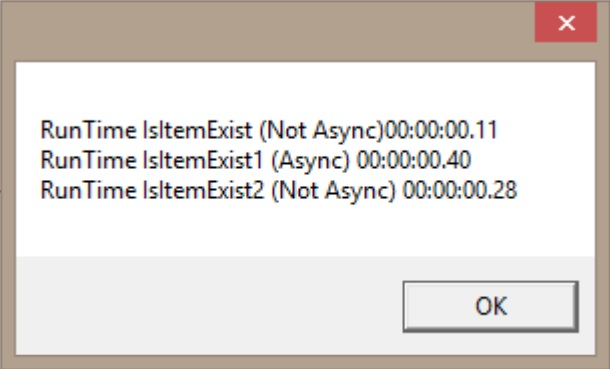
\includegraphics[width=0.5\textwidth]{5}
\centering
\caption{Window view in the constructor mode}
\end{figure}

However, this solution of the problem is not correct because on an another computer recourse to this directory can take more time, in this case list of elements will not be filled correct and it will lead to the incorrect work of the whole method.

For correctly fixing this drawback it is necessary to change all the work of Yandex.Disk SDK. Thus, the decission was made to create the call to the cloud through WebDAV protocol and to liquidate an asynchrony. Class have not got any user interface because of that we can liquidate an asynchrony.

It is necessary to use WebDAV protocol methods to create an interaction with the cloud:
\begin{itemize}
\item PUT - Uploads a file
\item GET - Downloads a file
\item MKCOL - Creating of a directory
\item COPY - Copying a file/folder
\item MOVE - Movement and renaming of a file/folder
\item DELETE - Deleting a file/folder
\item PROPFIND - Getting the properties of files/directories
\item PROPPATCH - Changing the properties of a file/directory
\end{itemize}

From listed methods we will need only 4 of them: PUT, GET, MKCOL, PROPFIND.

Classes HttpWebRequest and HttpWebResponse, which included in the .NET Framework from version 2.0, will be used because WebDAV uses HTTP/S. Class HttpWebRequest represents HTTP-request, second - HTTP-response. Namespace System.Net for working with network have to be included. It is necessary to generate the request correctly for understanding it by the WebDAV server.

Every method has its own parameters. Some of them are the same for all methods:
\begin{itemize}
\item Remote host address (https://webdav.yandex.ru/)
\item Authentication data. Yandex receives this data in two types: Basic - login and password; OAuth-token. For transmission these data the string is used: request.Headers["Authorization"] = "OAuth " + AccessToken.
\item The command that has to be executed, e.g. requet.Method="PUT"
\end{itemize}

The name of the directory, in which method must be executed, is added to the address of the host in case of execution method in directory other than root.

Creation of a new directory in the cloud, i.e. execution MKCOL method,does not requires any parameters except mandatory. WebDAV-protocol does not allow to create several subfolders in one request.If directory is already exists and request tries to create directory with the same name then exception, that must be handled, rises. To find out does directory exist, we can send a request for creating the directory and handle the exception with code 405 - "Invalid method", which raises in case of creation the directory with the same name.

Requestion the properties -PROPFIND method, does not requires any parameters except mandatory too. However, it is necessary to parse received response (XML format) from the server. Besides parsing the response, it is necessary to catch an exception with 404 code - "Element not found".

Unlike other methods, PUT and GET requires for an additional parameters, like variables for data reading and writing.

For example, in addition to setting variables, for method GET execution, we will need to get size of a file from the header, create file stream for writing a file on a local drive, receive the stream from the server. The next step is reading the data from received stream and writing them to the open stream. If amount of read bytes are equal to read from the header, then file downloading is succesfull.

For method PUT it is necessary to set parameters:
 \begin{itemize}
\item AllowWriteStreamBuffering - It enables or disables data buffering before sending it. If it is enable, then file loads to the memory, first, and only after that to the server.
\item SendChunked - It allows to upload files of uncertainsize to a remote host 
\item Expect100Continue - Parameter that includes waiting for a response from the server with code 100. It means that we can continue, in other casse its value will be false.
\end{itemize}

After completion formation of the query, it is necessary to receive a network flow where the data, which will be sent to the server, written in. We also need to open a local file for reading, allocate byte buffer for temporary storing data read from the file. Then read and send are produced in the cycle and data are written to the flow. Network and file flows are closed after that. HTTP status has to be checked for equality to the flag Created and to compared the size of the file with amount of sended bytes. Sending was succesfull if both of this conditions are fulfilled, else - there was an error.

After synchronous methods were written, the decision was taken to compare the time of their execution with asynchronous. The Stopwatch class is used for the precise measurement of time. To an object of TimeSpan class the measured time is assigned after measurements were finished. Measurement's results are presented on the poped up window in hh:mm:ss.ms format (Fig. 5).
\begin{figure}[h]
\centering
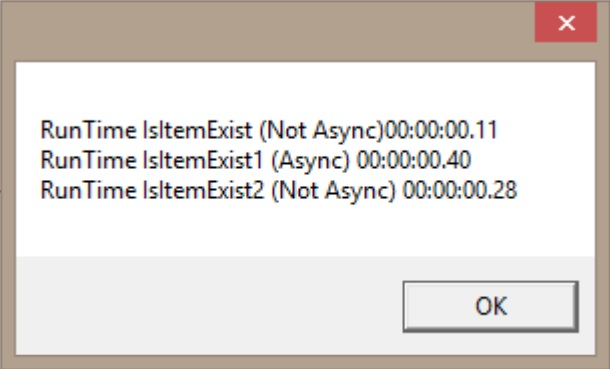
\includegraphics[width=0.5\textwidth]{6}
\centering
\caption{Measurement's results}
\end{figure}

According to the results, the best method for our targets is synchronous IsItemExist method.

Except downloading and uploading file to the server, it is necessary to organize the work with it. For example, the file have to be opened if it is an image. This method is realized in the OpenFile method, which downloads a file from the cloud and then opens it with LaunchFile method. We have to make sure that a user is finished working with it to delete a file, for this we show a window with a message. The file closes and deletes if the window was closed.

\section{Conclusion}
The software that allows user to take a snapshot of a document with web-camera and a scanned copy with scanner was developed during execution of this work. An ability of creation different acts based on MS Word and MS Excel templates was orginized. The work with files in the cloud was also orginized.

Each task cold be solved with different ways. The choise of methods depend from targets ans programmer choidse. For example, AForge.NET was selected for making a photos because of its simplicity in use and easy accessibility. TWAIN library, for working with scanner, was selected because of big amount of scanners are TWAIN-devices. This library is time-tested and reliable besides a lot of TWAIN projects in the Internet. Yandex.Disk was selected mostly because of personal experience.

The problem of lacking the video player WPF element was solved during the photo making task. The WindowsHost element, that allows to include a Windows Forms element into WPF, was used.

The decision to move from 64-bit (x64) on 32-bit(x84) version of software was made, because of 64-bit version is not supported by all TWAIN-compatible scanners.

The work with templates was complicated by an error that was accepted with Microsoft company. To avoid this error, the method, that could be executed with one string, must be devided into three strings. This solution was suggested by Microsoft.

It was determined that the work with Yandex.Disk will not be an optimal due to asynchronous. For the solution this defect, methods of appealing to the cloud server through WebDAV were created. At the end of the work measurements of execution synchronous and asynchronous methods were made. As was shown in the results, in this case, synchronous methods are faster.

We can conclude that all tasks were fully solved. The target of the creation the software as a subsystem for an ASC, that provides an automating of tasks related to the attached documents, was achieved.
\end{document}
